\chapter{Game Design and Algorithms}
\label{ch:game-design}

This chapter describes the core Minesweeper game engine, implemented as a
set of pure functions in \texttt{frontend/src/utils/minesweeper.js} and
driven by the stateful hook \texttt{useMinesweeper.js}. Because the game
engine is the technical core of this project, it is treated here as a
dedicated chapter rather than as a subsection of the general implementation
chapter.

\section{Board Representation}
The board is represented as a two-dimensional array of cell objects. Each
cell has four fields:
\begin{itemize}[nosep]
    \item \texttt{isMine} -- whether the cell contains a mine.
    \item \texttt{isRevealed} -- whether the cell has been uncovered.
    \item \texttt{isFlagged} -- whether the player has marked the cell.
    \item \texttt{adjacentMines} -- the count of mines among the cell's up
    to 8 neighbours.
\end{itemize}
\texttt{createEmptyBoard} builds this grid with every cell initialised to
safe, unrevealed, and unflagged, before any mines are placed.

\section{Difficulty Configuration}
Two difficulties are defined in a single configuration object,
\texttt{DIFFICULTIES}, shown in Table~\ref{tab:difficulties}. Centralising
these values avoids duplicating grid dimensions across components.

\begin{table}[h]
\centering
\caption{Supported difficulty configurations.}
\label{tab:difficulties}
\begin{tabular}{@{}lccc@{}}
\toprule
\textbf{Difficulty} & \textbf{Grid} & \textbf{Mines} & \textbf{Safe Cells} \\
\midrule
Beginner & $9 \times 9$   & 10 & 71 \\
Advanced & $16 \times 16$ & 40 & 216 \\
\bottomrule
\end{tabular}
\end{table}

\section{First-Click Safety}
\label{sec:first-click}
Mines are not placed when the board is created; they are placed only in
response to the player's first reveal, via \texttt{placeMines(board,
mineCount, safeRow, safeCol)}. The function first builds a set containing
the clicked cell and all of its neighbours (up to 8 cells), marking them as
off-limits to mine placement. It then builds a list of every remaining
candidate cell, shuffles it with a Fisher--Yates shuffle, and takes the
first \texttt{mineCount} cells from the shuffled list as mine positions.
Finally, it computes \texttt{adjacentMines} for every non-mine cell by
counting mines among its neighbours. This guarantees that a player's first
click, and the small neighbourhood around it, can never immediately end the
game.

\begin{lstlisting}[language=JavaScript, caption={Simplified first-click safety and mine placement (\texttt{minesweeper.js}).}, label={lst:place-mines}]
export function placeMines(board, mineCount, safeRow, safeCol) {
  const safeCells = new Set([`${safeRow},${safeCol}`]);
  getNeighbors(board, safeRow, safeCol).forEach((cell) => {
    safeCells.add(`${cell.row},${cell.col}`);
  });

  const candidates = [];
  for (let row = 0; row < board.length; row++) {
    for (let col = 0; col < board[0].length; col++) {
      if (!safeCells.has(`${row},${col}`)) candidates.push([row, col]);
    }
  }

  // Fisher-Yates shuffle
  for (let i = candidates.length - 1; i > 0; i--) {
    const j = Math.floor(Math.random() * (i + 1));
    [candidates[i], candidates[j]] = [candidates[j], candidates[i]];
  }

  const mineCells = candidates.slice(0, mineCount);
  // ... mark mineCells as isMine = true, then compute adjacentMines
}
\end{lstlisting}

\section{Flood-Fill Reveal Algorithm}
\label{sec:flood-fill}
When a cell with \texttt{adjacentMines === 0} is revealed, all of its
neighbours are safe to reveal automatically, and this cascades outward until
every reachable zero-adjacency region and its numbered border has been
uncovered. This is implemented in \texttt{revealCell(board, row, col)} using
an explicit stack rather than recursion, which avoids call-stack depth
concerns on larger boards such as the $16\times16$ Advanced grid. Each
iteration pops a coordinate, skips it if already revealed or flagged,
reveals it, and -- if it has zero adjacent mines and is not a mine -- pushes
its unrevealed, unflagged neighbours onto the stack for processing.

\begin{lstlisting}[language=JavaScript, caption={Iterative flood-fill reveal (\texttt{minesweeper.js}).}, label={lst:flood-fill}]
export function revealCell(board, row, col) {
  const newBoard = board.map((r) => r.map((cell) => ({ ...cell })));
  const stack = [[row, col]];

  while (stack.length > 0) {
    const [r, c] = stack.pop();
    const cell = newBoard[r][c];
    if (cell.isRevealed || cell.isFlagged) continue;
    cell.isRevealed = true;

    if (cell.adjacentMines === 0 && !cell.isMine) {
      getNeighbors(newBoard, r, c).forEach((neighbor) => {
        if (!neighbor.isRevealed && !neighbor.isFlagged) {
          stack.push([neighbor.row, neighbor.col]);
        }
      });
    }
  }
  return newBoard;
}
\end{lstlisting}

Figure~\ref{fig:flood-fill-example} illustrates a worked example: revealing
a single zero-adjacency cell cascades outward until it reaches cells with a
non-zero mine count, which are revealed but do not propagate further.

\begin{figure}[h]
\centering
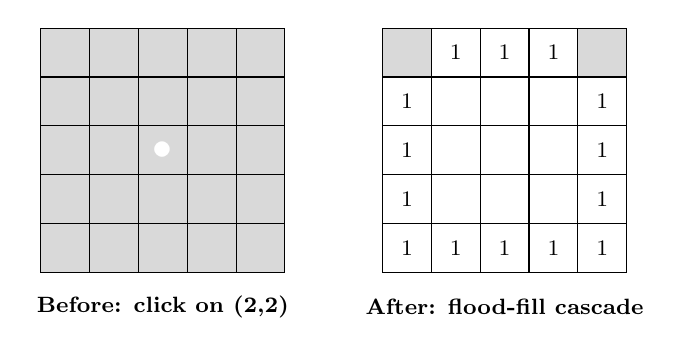
\begin{tikzpicture}[scale=0.62, every node/.style={font=\footnotesize}]
  % Before grid
  \begin{scope}
    \foreach \x in {0,...,4} {
      \foreach \y in {0,...,4} {
        \draw[fill=gray!30] (\x,\y) rectangle ++(1,1);
      }
    }
    \node at (2.5,-0.7) {\textbf{Before: click on (2,2)}};
    \node at (2.5,2.5) {\textcolor{white}{\Large $\bullet$}};
  \end{scope}
  % After grid
  \begin{scope}[xshift=7cm]
    \foreach \x in {0,...,4} {
      \foreach \y in {0,...,4} {
        \draw[fill=gray!30] (\x,\y) rectangle ++(1,1);
      }
    }
    % revealed cascade (zeros) - center cross region
    \foreach \x/\y in {1/1,2/1,3/1,1/2,2/2,3/2,1/3,2/3,3/3} {
      \draw[fill=white] (\x,\y) rectangle ++(1,1);
    }
    % bordering numbered cells: draw the white fills FIRST, then the
    % number labels on top, so the labels stay visible
    \draw[fill=white] (0,0) rectangle ++(1,1);
    \draw[fill=white] (0,1) rectangle ++(1,1);
    \draw[fill=white] (0,2) rectangle ++(1,1);
    \draw[fill=white] (0,3) rectangle ++(1,1);
    \draw[fill=white] (4,0) rectangle ++(1,1);
    \draw[fill=white] (4,1) rectangle ++(1,1);
    \draw[fill=white] (4,2) rectangle ++(1,1);
    \draw[fill=white] (4,3) rectangle ++(1,1);
    \draw[fill=white] (1,0) rectangle ++(1,1);
    \draw[fill=white] (2,0) rectangle ++(1,1);
    \draw[fill=white] (3,0) rectangle ++(1,1);
    \draw[fill=white] (1,4) rectangle ++(1,1);
    \draw[fill=white] (2,4) rectangle ++(1,1);
    \draw[fill=white] (3,4) rectangle ++(1,1);
    \node at (0.5,0.5) {1};
    \node at (0.5,1.5) {1};
    \node at (0.5,2.5) {1};
    \node at (0.5,3.5) {1};
    \node at (4.5,0.5) {1};
    \node at (4.5,1.5) {1};
    \node at (4.5,2.5) {1};
    \node at (4.5,3.5) {1};
    \node at (1.5,0.5) {1};
    \node at (2.5,0.5) {1};
    \node at (3.5,0.5) {1};
    \node at (1.5,4.5) {1};
    \node at (2.5,4.5) {1};
    \node at (3.5,4.5) {1};
    \node at (2.5,-0.7) {\textbf{After: flood-fill cascade}};
  \end{scope}
\end{tikzpicture}
\caption{Worked example of the flood-fill reveal: clicking a zero-adjacency
cell cascades to reveal the surrounding zero region and its numbered
border, while unrelated cells remain hidden.}
\label{fig:flood-fill-example}
\end{figure}

\section{Flagging}
\texttt{toggleFlag(board, row, col, mineCount)} toggles a cell's flag state.
A revealed cell cannot be flagged. A new flag is only placed if the current
number of flags on the board (\texttt{countFlags}) is below the mine count
for the active difficulty, preventing the flag counter from going negative
in the UI.

\section{Chording}
\label{sec:chording}
Chording lets the player reveal all unflagged neighbours of an
already-revealed numbered cell in one action, once the surrounding flags
match its number. \texttt{chordCell(board, row, col)} first checks that the
target cell is revealed, has a non-zero \texttt{adjacentMines} value, and is
not itself a mine. It then counts flagged neighbours; if that count does not
equal \texttt{adjacentMines}, the board is returned unchanged. Otherwise,
every unflagged, unrevealed neighbour is revealed via \texttt{revealCell}
(triggering flood-fill where applicable). If a chord reveals a mine -- i.e.\
the player mis-flagged -- the calling code in \texttt{useMinesweeper}
detects a revealed mine cell in the resulting board and ends the game.

\begin{lstlisting}[language=JavaScript, caption={Chording logic (\texttt{minesweeper.js}).}, label={lst:chord}]
export function chordCell(board, row, col) {
  const cell = board[row][col];
  if (!cell.isRevealed || cell.adjacentMines === 0 || cell.isMine) return board;

  const neighbors = getNeighbors(board, row, col);
  const adjacentFlagCount = neighbors.filter((n) => n.isFlagged).length;
  if (adjacentFlagCount !== cell.adjacentMines) return board;

  let workingBoard = board;
  neighbors
    .filter((n) => !n.isFlagged && !n.isRevealed)
    .forEach((n) => { workingBoard = revealCell(workingBoard, n.row, n.col); });
  return workingBoard;
}
\end{lstlisting}

\section{Hint System}
\texttt{findHintCell(board)} collects every cell that is not a mine, not
revealed, and not flagged, and returns one at random. The calling hook
records the hint usage (capped at \texttt{MAX\_HINTS = 3}), stores the
returned coordinates as the currently highlighted \texttt{hintCell}, and
clears the highlight after \texttt{HINT\_HIGHLIGHT\_MS = 3000} milliseconds
via a timeout. Each hint used subtracts \texttt{HINT\_COST = 50} points from
the eventual score (Section~\ref{sec:scoring}).

\section{Shield Ability}
Each game grants the player exactly one shield, tracked as a three-state
value: \texttt{available}, \texttt{active}, and \texttt{used}. Activating
the shield (\texttt{activateShield}) is only permitted while it is
\texttt{available}. While \texttt{active}, the next time the player reveals
a mine, \texttt{revealCellAt} sets the shield to \texttt{used} and returns
without ending the game or revealing the mine, letting play continue.
Figure~\ref{fig:shield-state} shows the shield's state machine. Note that
because mines are placed only on the first click
(Section~\ref{sec:first-click}), an active shield can, in principle, be
consumed by the very first reveal if that reveal happens to land on a
mine-designated cell outside the guaranteed-safe neighbourhood -- though in
practice first-click safety makes this impossible for the first click
itself, and the shield instead protects the player's first mine encounter
on any later click.

\begin{figure}[htbp]
\centering
\begin{tikzpicture}[node distance=4.2cm, on grid, auto,
    every state/.style={minimum size=1.6cm}]
  \node[state, initial, fill=green!15] (avail) {available};
  \node[state, right=of avail, fill=cyan!15] (active) {active};
  \node[state, right=of active, fill=gray!20] (used) {used};

  \path[-{Latex[length=2.5mm]}]
    (avail) edge node[above, text width=2.2cm, align=center] {activate} (active)
    (active) edge node[above, text width=2.6cm, align=center] {mine revealed} (used);
\end{tikzpicture}
\caption{Shield ability state machine.}
\label{fig:shield-state}
\end{figure}

\section{Game State Machine}
The overall game progresses through three states, tracked as
\texttt{gameStatus} in \texttt{useMinesweeper}: \texttt{ready} (board
created but mines not yet placed), \texttt{playing} (first click made,
timer running), and \texttt{lost} (a mine was revealed without an active
shield, or the timer reached zero). There is deliberately no
\texttt{won}/\texttt{completed-board} state.

\begin{figure}[htbp]
\centering
\begin{tikzpicture}[node distance=4.6cm, on grid, auto,
    every state/.style={minimum size=1.8cm}]
  \node[state, initial, fill=yellow!15] (ready) {ready};
  \node[state, right=of ready, fill=cyan!15] (playing) {playing};
  \node[state, right=of playing, fill=red!15] (lost) {lost};

  \path[-{Latex[length=2.5mm]}]
    (ready) edge node[above, text width=2.4cm, align=center] {first reveal} (playing)
    (playing) edge[bend left=35] node[above, text width=3.2cm, align=center] {mine hit (no shield)} (lost)
    (playing) edge[bend right=35] node[below, text width=2.6cm, align=center] {timer reaches 0} (lost);
\end{tikzpicture}
\caption{Game status state machine. There is no explicit ``won'' state; the
game is a timed survival mode.}
\label{fig:game-state}
\end{figure}

\section{Survival Mode and the Absence of a Win Condition}
Every game begins with a fixed countdown of \texttt{TIME\_LIMIT\_SECONDS =
120}. The game does not end when all safe cells are revealed; the player may
continue revealing cells (subject to normal Minesweeper deduction) until
either a mine is hit or the timer expires. This design choice is reflected
in the database schema (Chapter~\ref{ch:database}), which stores
\texttt{cells\_revealed} and \texttt{time\_taken} but has no
\texttt{result}/win-loss column -- an explicit migration
(\texttt{migration-remove-win-condition.sql}) removed a previous
\texttt{result} column when survival mode was adopted.

\section{Scoring Formula}
\label{sec:scoring}
The score for a completed game is:
\[
\text{score} = \max\bigl(0,\; (\text{cellsRevealed} \times 10) +
(\text{timeElapsed} \times 0) - (\text{hintsUsed} \times 50)\bigr)
\]
\texttt{POINTS\_PER\_SECOND} is deliberately set to \texttt{0}. Although the
constant exists in the formula, it is defined as zero specifically to
prevent a player from inflating their score simply by surviving passively
(e.g.\ letting the timer run without revealing cells); the score is driven
entirely by the number of safe cells actually revealed, less a fixed penalty
per hint used. The same formula is evaluated twice: once on the client for
immediate UI feedback (\texttt{calculateScore} in \texttt{minesweeper.js}),
and independently on the server when the result is saved
(Section~\ref{sec:score-validation}), so that the value shown to the player
during play is never the value actually trusted for the leaderboard.

\begin{lstlisting}[language=JavaScript, caption={Client-side score formula (\texttt{minesweeper.js}).}, label={lst:score}]
export const POINTS_PER_CELL = 10;
export const POINTS_PER_SECOND = 0;
export const HINT_COST = 50;

export function calculateScore(cellsRevealed, timeElapsed, hintsUsed) {
  const rawScore = cellsRevealed * POINTS_PER_CELL
                  + timeElapsed * POINTS_PER_SECOND
                  - hintsUsed * HINT_COST;
  return Math.max(0, rawScore);
}
\end{lstlisting}

\section{Decision Flow of a Cell Reveal}
Figure~\ref{fig:reveal-flow} summarises the decision logic executed each
time the player clicks a cell, as implemented in \texttt{revealCellAt}
within \texttt{useMinesweeper.js}.

\begin{figure}[p]
\centering
\begin{tikzpicture}[every node/.style={font=\scriptsize}]
  \tikzstyle{decision} = [diamond, draw, fill=blue!10, text width=1.9cm,
      align=center, inner sep=1pt]
  \tikzstyle{action} = [rectangle, draw, fill=orange!15, text width=2.3cm,
      align=center, rounded corners]
  \tikzstyle{arrow} = [-{Latex[length=2mm]}, thick]

  % Column x-positions: A = main spine, B = first branch column,
  % C = second branch column. Rows are spaced generously (3.1cm) so that
  % the wide diamond shapes never touch their neighbours.
  \node (start)      [action]              at (0,0)      {Player clicks cell};
  \node (lostcheck)  [decision]            at (0,-2.6)    {Game already lost?};
  \node (stop1)      [action]              at (4.4,-2.6)  {Ignore click};
  \node (statecheck) [decision]            at (0,-5.8)    {Revealed or flagged?};
  \node (stop2)      [action]              at (4.4,-5.8)  {Ignore click};
  \node (readycheck) [decision]            at (0,-9.0)    {Status = ready?};
  \node (place)      [action]              at (4.4,-9.0)  {Place mines (first-click safe)};
  \node (minecheck)  [decision]            at (0,-12.4)   {Cell is a mine?};
  \node (shieldcheck)[decision]            at (4.9,-12.4) {Shield active?};
  \node (lose)       [action]              at (9.6,-12.4) {Reveal all mines, status = lost};
  \node (reveal)     [action]              at (0,-15.4)   {Flood-fill reveal cell};
  \node (consume)    [action]              at (4.9,-15.4) {Consume shield, continue};

  \draw[arrow] (start) -- (lostcheck);
  \draw[arrow] (lostcheck) -- node[above] {yes} (stop1);
  \draw[arrow] (lostcheck) -- node[left] {no} (statecheck);
  \draw[arrow] (statecheck) -- node[above] {yes} (stop2);
  \draw[arrow] (statecheck) -- node[left] {no} (readycheck);
  \draw[arrow] (readycheck) -- node[above] {yes} (place);
  \draw[arrow] (readycheck) -- node[left] {no} (minecheck);
  % Feedback path from "place mines" back into the main spine: dips down
  % in the empty gap between column A and column B, well clear of the
  % "Shield active?" diamond, before entering minecheck from the top.
  \draw[arrow] (place.south) -- ++(0,-1.6) -| (minecheck.north);
  \draw[arrow] (minecheck) -- node[above] {yes} (shieldcheck);
  \draw[arrow] (minecheck) -- node[left] {no} (reveal);
  \draw[arrow] (shieldcheck) -- node[above] {no} (lose);
  \draw[arrow] (shieldcheck) -- node[left] {yes} (consume);
\end{tikzpicture}
\caption{Decision flow for handling a cell reveal in \texttt{revealCellAt}.}
\label{fig:reveal-flow}
\end{figure}
